\subsection{Model}

We have developed a fluid model of TIMELY, as shown in
Tables~\ref{tab:timely_var} and \ref{tab:timely_param} and
Figure~\ref{fig:timely_model}.  The model considers N flows, traversing a single
bottleneck link. The model assumes that TIMELY is triggered
before\footnote{Unlike~\cite{dcqcn}, ~\cite{timely} does not specify how to set
buffers to ensure this, but we assume that it can be done.} PFC, and hence
ignores the impact of PFC.

Equation~\ref{eq:timely_q} describes the queue behavior.
Equation~\ref{eq:timely_r} describes rate computation. For simplicity, we ignore
the hyperactive increase phase. When RTT is between$T_{low}$ and $T_{high}$, the
rate computation depend on RTT gradient, which evolves according to
Equation~\ref{eq:timely_g}.  The equation captures the EWMA filter, as well as
normalization. Since the gradient is the difference between the current and the
previous RTT sample, it depends on two queue lengths in past: one at time $t -
\tau'$, and one at time $t - \tau'-\tau\*$. The value of $\tau'$ and $\tau*$
depend on past transmission rates, but to simplify the model, we approximate
their calculation as shown in Equations~\ref{eq:timely_taus} and
\ref{eq:timely_taup}.  Equation~\ref{eq:timely_taus} captures the fact that the
TIMELY implementation updates rate at most once per $D_{minRTT}$.

\begin{table}[t]
\center
{
\footnotesize
{
\begin{tabular}{|c|c|} \hline
Variable & Description \\ \hline
$R$ & Rate \\ \hline
$g$ & RTT gradient\\ \hline
$q$ & Queue Size \\ \hline
$t$ & Time \\ \hline
$\tau*$ & Rate update interval \\ \hline
$\tau'$ & Feedback delay \\ \hline
\end{tabular}
}
}
\caption{TIMELY Fluid model variables}
\label{tab:timely_var}
\end{table}

\begin{table}[t]
\center
{
\footnotesize
{
\begin{tabular}{|c|c|} \hline
Parameter & Description \\ \hline
$N$ & Number of flows at bottleneck\\ \hline
$C$ & Bandwidth of bottleneck link\\ \hline
$\alpha$ & EWMA smoothing factor\\ \hline
$\delta$ & Additive increase step\\ \hline
$\beta$ & Multiplicative decrease factor\\ \hline
$T_{low}$ & Low threshold\\ \hline
$T_{high}$ & High threshold\\ \hline
$D_{minRTT}$ & Minimum RTT for normalization \\ \hline
$D_{prop}$ & Propagation delay \\ \hline
\end{tabular}
}
}
\caption{TIMELY Fluid model parameters}
\label{tab:timely_param}
\end{table}

\begin{figure}[h]
\fbox
{
\begin{minipage}{\columnwidth}
\begin{equation}
\small
\frac{{dq}}{{dt}} = \sum_{i} R_i(t) - C\\
\label{eq:timely_q}
\end{equation}
\begin{equation}
\small
\frac{{dR_i}}{{dt}} = \left\{ \begin{array}{ll}
\frac{\delta }{{\tau *}}, & q(t - \tau ') < C*{T_{low}}\\
\frac{\delta }{{\tau *}}, & g \le 0\\
 - \frac{{g\beta }}{{\tau *}}R_i(t), & g > 0\\
 - \frac{\beta }{{\tau *}}(1 - \frac{{C*{T_{high}}}}{{q(t - \tau ')}})R_i(t), & q(t - \tau ') > C*{T_{high}}
\end{array} \right.\\
\label{eq:timely_r}
\end{equation}
\begin{equation}
\small
\frac{{dg}}{{dt}} = \frac{\alpha }{{\tau *}}( - g(t) + \frac{{q(t - \tau ') - q(t - \tau ' - \tau *)}}{{C*{D_{\min RTT}}}})\\
\label{eq:timely_g}
\end{equation}
\begin{equation}
\small
\tau * = \max \{ \frac{{Seg}}{R},{D_{\min RTT}}\} \\
\label{eq:timely_taus}
\end{equation}
\begin{equation}
\small
\tau ' = \frac{q}{C} + \frac{{Seg}}{C} + {D_{prop}}
\label{eq:timely_taup}
\end{equation}
\end{minipage}
}
\caption{TIMELY fluid model}
\label{fig:timely_model}
\end{figure}

\para{Model Validation:}
Since we do not have access to TIMELY implemenation,
Figure~\ref{fig:timely_model_validation} compares the TIMELY fluid model with
the packet-level simulations using the NS3 simulator~\cite{ns3}. The parameters
values are shown in Table~\ref{tab:timely_model_validation}, and are based on
guidance provided in\cite{timely}.  We model a simple topology, in which N
senders, connected to a switch, send to a single receiver, also connected to
that switch. The starting rate for each flow is set to be 1/N of the link
bandwidth. 

We see the fluid model and the simulator are in good agreement, apart from some
time shift in queue behavior. The queue peaks at roughly 70KB, which corresponds
to 56$\mu$s at 10Gbps. As one would expect, this is close to the $T_{min}$.

\begin{table}[t]
\small
\center
\begin{tabular}{c|c}
Parameter & Value \\ \hline
C & 10Gbps \\ 
$T_{low}$ & 50 $\mu$s \\ 
$T_{high}$ & 500 $\mu$s \\
$D_{minRTT}$ & 20 $\mu$s \\
$\beta$ & 0.8 \\
$\alpha$ & 0.875 \\
$\delta$ & 10Mbps
\end{tabular}
\caption{TIMELY parameter values for model validation}
\label{tab:timely_model_validation}
\end{table}

\begin{figure*}[t]
\center
\subfigure[N=2] { 
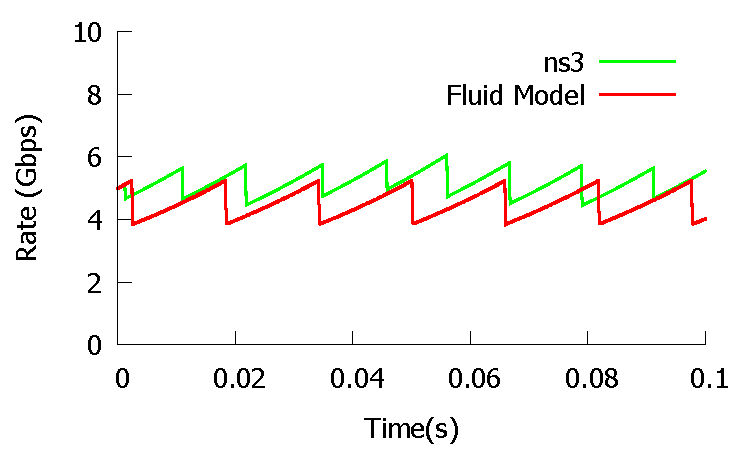
\includegraphics[width=0.3\textwidth]{figures/timely_validation_2_rate.pdf}
}
\subfigure[N=10] { 
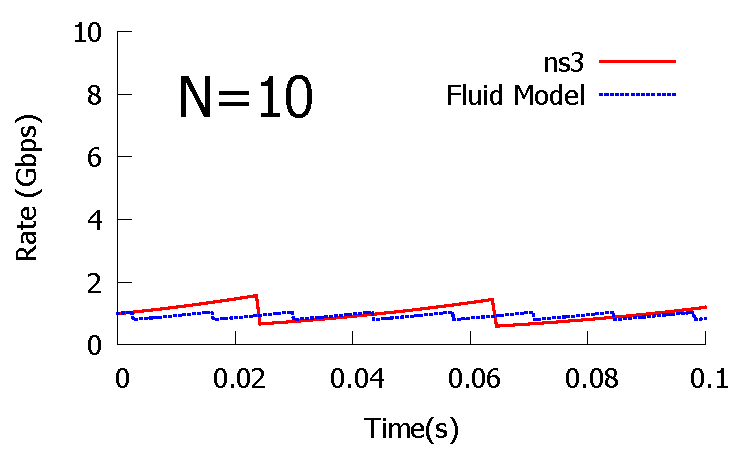
\includegraphics[width=0.3\textwidth]{figures/timely_validation_10_rate.pdf}
}
\subfigure[N=20] { 
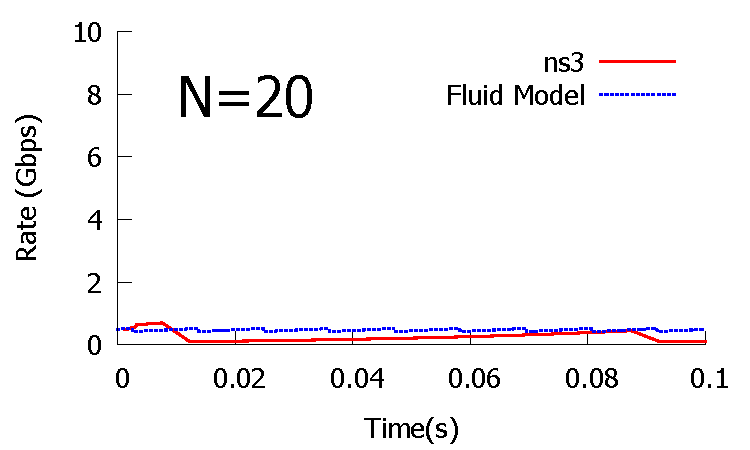
\includegraphics[width=0.3\textwidth]{figures/timely_validation_20_rate.pdf}
}
\caption{Comparison of TIMELY fluid model and simulations}
\label{fig:timely_model_validation}
\end{figure*}

